\documentclass[12pt]{article}
\usepackage{fullpage}
\subsectionfont{\fontfamily{phv}\fontsize{13pt}{13pt}\selectfont}
%\newcommand{\var}[1]{\mathit{#1}}
\usepackage[margin=1cm]{geometry}
\usepackage{amsmath}
\usepackage{graphicx}
\usepackage{listings}
\begin{document}
\begin{titlepage}
\newcommand{\HRule}{\rule{\linewidth}{0.5mm}} % Defines a new command for the horizontal lines, change thickness here
\center % Center everything on the page
%----------------------------------------------------------------------------------------
% HEADING SECTIONS
%----------------------------------------------------------------------------------------
\HRule \\[0.4cm]
{ \huge \bfseries Phase 2}\\[0.4cm] % Title of your document
\HRule \\[1.5cm]
\begin{minipage}{0.4\textwidth}
\begin{center} \large
Programming on the Web\\
CSC309H1, Winter 2015\\
\today
\end{center}
\end{minipage}
\vfill % Fill the rest of the page with whitespace
Cody Rosevear, c3roseve\\
999499332\\
\\
Denis Marchin, g3dmarch\\
999061009\\
\\
Farzad Hemmati, c3hemmat\\
999964953\\
\\
Akira Kakkar, g3fol\\
999825541\\
\\
\end{titlepage}
\newpage
\section*{Description}
\begin{enumerate}

\item[0.]

\textbf{URL}
http://104.236.231.174/

\textbf{Phase3 Code Snapshot}
https://mega.co.nz/#!EoMWhYoJ!k3MZ6tYcm-0HXnZOH4bv7oAG-jG89aZ3ozhByB2r1U8

\item[1.] Feature and Functionality Specification

\textbf{Homepage}

-Login button

-Register button

-Browse button

-Create button

\textbf{Register Page}
-Email box

-Password box

-Re-enter password box

\textbf{Profile page}

-Profile picture

-Name

-Reputation score as funder and as initiator

-Initiated projects list

-Funded projects list

-Bio

-Skills/Experience (maybe)

\textbf{Browse projects page}

-Search bar

-Pre-made filters for various project rankings(ex: most funded, closest to goal, high reviews etc...)

-Category button to filter by project categories (within a user's communities)

\textbf{Browse community page}

-Search bar

-Subscribe button to join a community once found.

\textbf{Create project page}

-Project name box

-Funding goal box

-Description box

-Pitch video (maybe)

-Funding perks box

-Project initiator  box

\textbf{Project page}

-All of the information from the create project page

-Fund button

-Project Review section (to comment on and rate projects)

-Reviews can also be rated by other users for their usefullness

\textbf{Fund page}

-Funding amount entry box

-Payment method selection box

\textbf{Admin page}

-Total number of projects

-Total number of projects funded

-Average time to reach a funding goal

\begin{figure}[ht!]
\centering
\includegraphics[width=200mm]{flowchart1.pdf}
\caption{Website Flowchart \label{overflow}}
\end{figure}


\item[2.] Project Plan

\textbf{General protocol}

Communication:Weekly meetings will occur on wednesday's before class to discuss any issues related to development and write the weekly report. Moreover, Skype and Facebook will serve as methods of contact for resolving any immediate issues.

Team Roles: These will be contingent on the phase of development, and assigned for the given week at each weekly meeting. To be decided: We may segregate the team into front-end and back-end specializations.

Problem resolution: All decisions are made democratically by vote.

\textbf{Milestones}

Note 1: The following schedule is ordered according to the perceived dependencies of the various features of the website. First the raw skeletons, then the database underlying all of the website information, followed by suitable integration between the database and web pages so that they display all of their content properly. Then, the more dynamic functionality is built weekly on top of this static base. 

Week1: Page skeletons, links, and basic styling

Week2: Central Database design and query development for all pages that use said database.

Week3: Project/Community/Profile page information is integrated with the database such that the pages display accurately.

Week4: Search functionality for all types of pages is operational.

Week5: Review System

Week6: Payment System

Week7: Admin Analytics

Week8: Additional Debuggging and Development Overflow

\item[3.] Software Architecture and High-level Design
\begin{figure}[ht!]
\centering
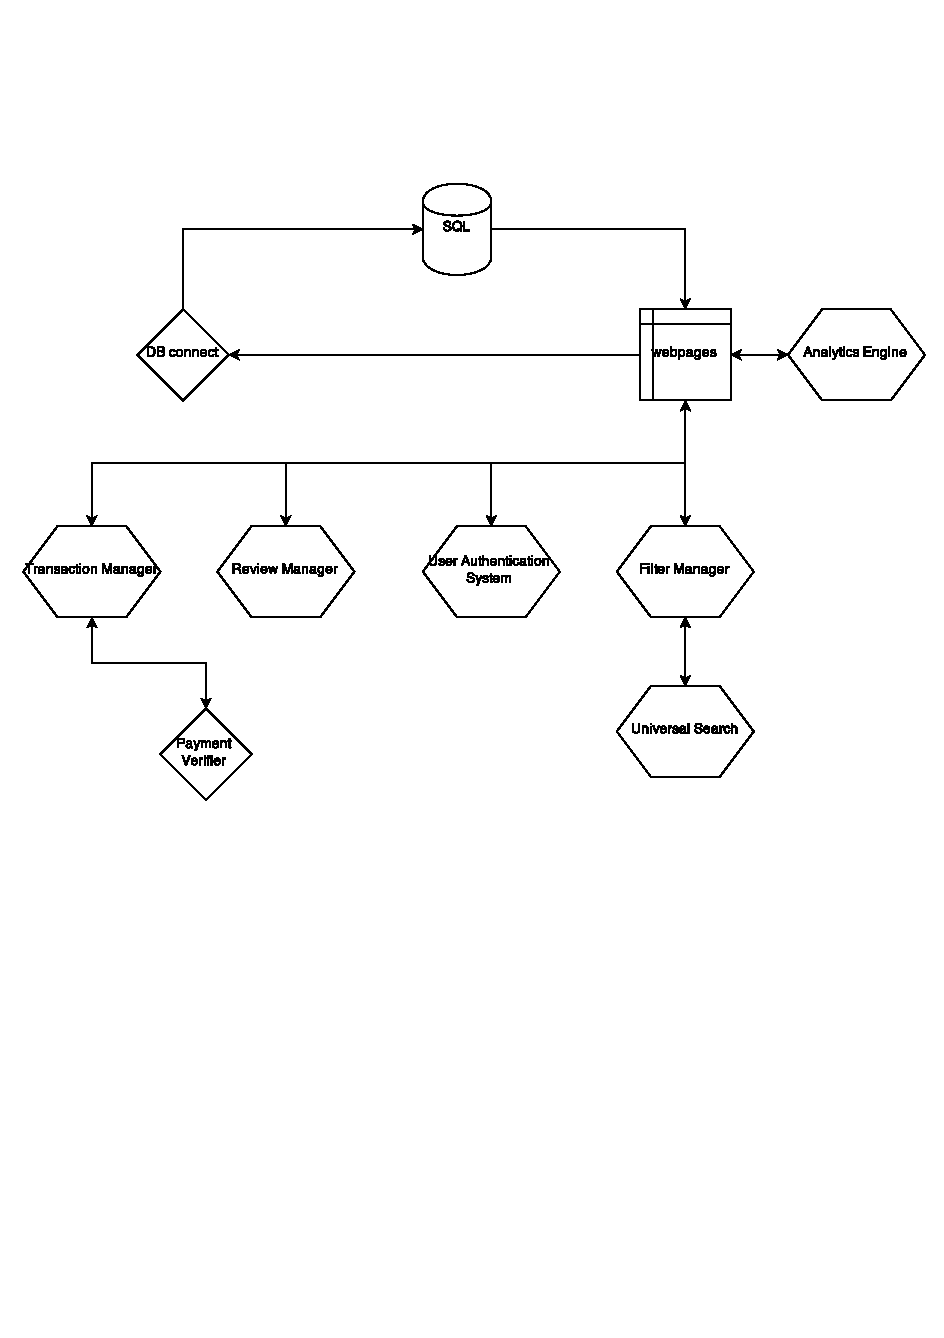
\includegraphics[width=150mm]{swag.pdf}
\caption{Software Components \label{overflow}}
\end{figure}

We are using PHP as our server-side language. For our front-end we will be using Javascript and JQuery. For our html and css design, we are going to be using bootstrap3.

We will have a central MySql database which keeps track of all the data associated with each of the various webpages. This will be the central repository from which all of the information webpages will request information when displaying webpages to users. It will also serve as the storehouse for transaction logging.

We will also have a database connector module that will be used by all of the webpages, so as to avoid code duplication.

All of the individual manager components are subsets of the functionality of the webpages themselves, and are therefore connected to the central database inasmuch as the webpages are connected to it.

The filter manager is the core software componenet that subserves all of the search functionality of the browse pages (both project and community). The filter manager will, in effect, be a more specialized instance of the code utilized for universal search throughout the website.

The transaction manager will require interaction with the central repository, since transactions will be logged in addition to processed. It will, of course, have a subfunction that verifies the payement by interacting with a third party (Paypal/credit card company).

The review manager provides the functionality to each project page which allows for funders to comment on projects as well as the reviews of other funders. It will need to be decomposed into both a rating system as well as a comment system.

The admin analytics componentt subserves the unique features of the admin view. It interacts with the central database, using the data stored there to compute statistics. This will need to be further decomposed into various functions that compute said statistics.

In terms of errors, we will display the corresponding error to the user. If the database is down and a user tries to access it, we will report to the user that database servers are down. All of this is already implemented for phase 3.


Finally, the user authentication system will be utilized wherever any kind of authentication is necessary. Since the process should generally be the same irrespective of the reason for authentication, it can be modularized.


\item[4.] Information Representation\\
User(\underline{userId} name, email, dob, password)\\
Transaction(\underline{user}, \underline{project}, \underline{date}, amount)\\
Communities(\underline{cId}, \underline{project})\\
Project(\underline{pId}, name, description, date, creator, totalAmount, community)\\
Review(\underline{project}, \underline{rate})\\
MemberOf(\underline{community}, \underline{user})\\
\\
Project(creator) \subseteq User(userId)\\
Transaction(user) \subseteq User(userId)\\
MemberOf(user) \subseteq User(userId)\\
Review(project) \subseteq Project(pId)\\
Transaction(project) \subseteq Project(pId)\\
Community(project) \subseteq Project(pId)\\
MemberOf(community) \subseteq Communities(cId)\\
Project(community) \subseteq Communities(cId)\\

\item[5.] Test Strategy and Test Plan

Just as project initiators on this site will test their ideas and creations, we will be testing the website. Hard staff responsibilities will be assigned on a weekly basis. All team members are responsible for testing the website. Website builders are expected to do some level of testing as they create a feature. Thorough testing of the feature from as many angles as possible will be completed nearer the end of the project phase. Website additions are expected to be tested for basic working functionality. Basic testing should be done in a timely manner, and before starting new feature additions. Record keeping of testing will take place. GitHub will be used to store the group’s file assets. Untested, and therefor possibly broken additions, should be marked as such in the commit message. Features that have been tested to work properly will also be marked as such in the commit message. At our weekly meetings, team members are expected to give a report update on what testing they have completed that week, and we will distribute the new testing tasks.

The testing of the website will be broken down into 4 main sections: database, UI, search, and transactions. The user interface will need to be tested. We want the website to feel intuitive and easy to use. We do not want to discourage users by having a steep learning curve. As the webpages are built, the layout and navigation will be tested for user friendliness. Near the end of the project phase, we will illicit our peers to test the website for ease of use. Payments for projects will need to be tested. Test projects and profiles will be created to send actual funds to a project. We will integrate the established payment system of Paypal. However robust the PayPal system may be, as users of their product, we should be familiar with its operation, including making test scenarios. The major testing anticipated is for the databases. Queries will be tested for correctness. We need to ensure data is received correctly and is outputted correctly. Security is an extremely important element to test. We will be storing sensitive data in our database, such as passwords and emails, and have a responsibility to protect the data of our users. Test databases will be created to simulate the site being operational, with many users, communities, projects, and their interactions. Common security flaws will be assessed and tested against, such as SQL injection. Data validation will be extensively tested, with test cases to guarantee only appropriate data in accepted. Users will be able to search for project using various categories. Unit testing will be used to test the site’s search function. Each type of search will be tested, and will use a test database to search against. Creating not only a working site, but an enticing one, through the process of thorough testing will give this site the potential for popularity.

\end{enumerate}
\end{document}